\documentclass[a4paper,11pt]{article}
\usepackage{fullpage}

\input{macros}

\newcommand{\Timeout}{600.00} % CPU seconds

\title{\textbf{Constraint Programming (course 1DL440) \\
    Uppsala University -- Autumn 2013 \\
    Report for Assignment $n$ / Project Part $n$  % replace n by 1, 2, or 3
    by Team $t$  % replace t by your team number
  }
}

\author{Clara CLEVER \and Whiz KIDD} % replace by your name(s)

%\date{Month Day, Year}
\date{\today}

\begin{document}

\maketitle

\noindent
This document shows the ingredients of a good homework report for the
CP course.  The \LaTeX\ source code of this document exemplifies
almost everything you need to know about \LaTeX\ in order to typeset a
professional-looking homework report (for the CP course).  Use it as a
starting point for imitation and delete everything irrelevant.  The
usage of \LaTeX\ is \stressed{optional}, but highly recommended, for
reasons that will soon become clear to those who have never used it
before; any learning time is \stressed{outside} the budget of this
course, but will hugely pay off, if not in this course then in the
next course(s) you take and when writing your BSc, MSc, or PhD thesis.

\section{The Sudoku Problem}
\label{sec:sudoku}

\subsection{Model}

\newcommand{\Hints}{\textit{Hints}}
\newcommand{\Sudoku}{\textit{Sudoku}}

\paragraph{Instance Data and Derived Constants.}
\begin{itemize}
\item $n$ designates the number of cells along one side of the
  generalised Sudoku board.  Hence there are $n^2$~cells in total.  We
  assume that $\sqrt{n}$ is an integer.
\item $N$ designates the set~$\Set{1,2,3,\dots,n}$.
\item $N'$ designates the set
  $\Set{0,\sqrt{n},2\cdot\sqrt{n},\dots,n-\sqrt{n}}$.
\item $\Hints$ designates the set of hints of the Sudoku board that is
  to be completed.  Each hint takes the form~$\Tuple{r,c,v}$, meaning
  that the cell at row~$r$ and column~$c$ takes value~$v$, with $r,c,v
  \in N$.
\end{itemize}

\paragraph{Decision Variables.}
\begin{itemize}
\item $\Sudoku[r,c]$ designates the value of the cell at row~$r$ and
  column~$c$ of the Sudoku board, with $r,c \in N$.
  Hence~$\Domain{\Sudoku[r,c]} = N$.
\end{itemize}

\paragraph{Problem Constraints.}
\begin{itemize}
\item \emph{Row constraints} require the values in each row of the
  Sudoku board to be pairwise different:
  \begin{equation} \label{cons:row}
    \ForAll r \In N :
    \Distinct(\Sudoku[r,\star])
  \end{equation}
\item \emph{Column constraints} require the values in each column of
  the Sudoku board to be pairwise different:
  \begin{equation} \label{cons:col}
    \ForAll c \In N :
    \Distinct(\Sudoku[\star,c])
  \end{equation}
\item \emph{Block constraints} require the values in each block of the
  Sudoku board to be pairwise different:
  \begin{equation} \label{cons:block}
    \ForAll r,c \In N' :
    \Distinct(\Sudoku[r+1\dots\sqrt{n},c+1\dots\sqrt{n}])
  \end{equation}
\item \emph{Hint constraints} require the given hints to be satisfied:
  \begin{equation} \label{cons:hint}
    \ForAll \Tuple{r,c,v} \In \Hints :
    \Sudoku[r,c] = v
  \end{equation}
\end{itemize}
None of the problem constraints is enforced automatically by the
choice of decision variables.  We advocate enforcing domain
consistency on the constraints~(\ref{cons:row}) to~(\ref{cons:block}),
because \dots.  The hint constraints~(\ref{cons:hint}) are subsumed
upon their first run under any consistency level.

\paragraph{Objective Function.}  The Sudoku puzzle is a constraint
\emph{satisfaction} problem, hence there is no objective function to
be minimised or maximised.

\paragraph{Redundant Decision Variables.}  Our model has no redundant
decision variables, because \dots.

\paragraph{Channelling Constraints.}  Our model has no channelling
constraints, because \dots.

\paragraph{Implied Constraints.}  Our model has no implied
constraints, because \dots.

\paragraph{Symmetry-Breaking Constraints.}  Our model has no
symmetry-breaking constraints, because \dots.

\paragraph{Branching Heuristics.}  We will experiment with two
variable selection heuristics:
\begin{itemize}
\item \emph{Size\_Min}: Branch on an unassigned decision
  variable~$\Sudoku[r,c]$ with the smallest domain, ties being broken
  by the lexicographically smallest coordinate~$\Tuple{r,c}$.
\item \emph{None}: Branch on the unassigned decision
  variable~$\Sudoku[r,c]$ with the lexicographically smallest
  coordinate~$\Tuple{r,c}$.
\end{itemize}
In both cases, we use the \emph{Min} value selection heuristic to pick
the smallest value, say~$m$, in the domain of the chosen
variable~$\Sudoku[r,c]$.  We branch with $\Sudoku[r,c] = m$ in the
left branch and $\Sudoku[r,c] \neq m$ in the right branch.  We
advocate these branching heuristics, because \dots.

\paragraph{Exploration Order.}  We advocate exploring the search tree
in depth-first order, because \dots.

\subsection{Implementation}

A \Gecode~\cite{Gecode} implementation of the described model is
attached as file \texttt{sudoku.cpp}.

\paragraph{Compilation and Running Instructions.} \dots.  (Explain how
to run the implementation for a particular problem
instance~$\Tuple{n,\Hints}$ as well as particular consistency,
branching, and exploration choices.  This will help the teachers grade
your program.)

\paragraph{Sample Test-Run Commands.} \dots.  (Show sample inputs and
outputs, and check whether these test runs are reproducible by the
program you submit!)

\subsection{Experiments}

Our experiments were run under Linux OpenSuse~11.3 (64~bit) on an
Intel Core~i7~950 of 3.07~GHz with an 8~MB L2 cache and a 3~GB RAM.

\paragraph{Hint:}
First do \texttt{uname -a} (under Linux or Solaris) and then do
\texttt{more /proc/cupping} (Linux) or
\texttt{/usr/platform/$X$/sbin/prtdiag} (Solaris, where $X$ is the
last field in the reply of the previous command) to find this
information.  Mac OS X users find this information via ``About this
Mac'' in the Apple menu.  \bigskip

Table~\ref{tab:res:queens} gives the total runtime (in seconds) and
number of failures for $100$~$\Hints$ sets (available at \dots) each
for various values of~$n$, under the two branching heuristics.  The
time-out was $\Timeout$~seconds.  We observe that \emph{Size\_Min} +
\emph{Min} outperforms \emph{None} + \emph{Min} on all instances.  The
reason for this is that \dots.

\begin{table}[t]
  \centering
  \begin{tabular}{|r||r|r||r|r|} % use right alignment to achieve
                                 % decimal point alignment
    \hline
    & \multicolumn{2}{|c||}{\emph{Size\_Min} + \emph{Min}} &
    \multicolumn{2}{|c|}{\emph{None} + \emph{Min}} \\
    \cline{2-5}
    $n$ & Time (sec) & Failures & Time (sec) & Failures \\
    \hline
    \input{results.tex} % let your experiment script write directly
                        % into this file, making sure every number
                        % in a column has the same number of decimals
    \hline
  \end{tabular}
  \caption{Total runtime (in seconds) and number of failures in terms
    of~$n$, for $100$~$\Hints$ sets each}
  \label{tab:res:queens}
\end{table}

\paragraph{Hint:}
In order to save a lot of time, it is very important that you write
programs that conduct the experiments for you and directly generate
result tables (see the \LaTeX\ source code of
Table~\ref{tab:res:queens}) or plots, which are automatically imported
(rather than copied) into your report.

\section*{Intellectual Property}

We certify that this report and all its attachments are solely
produced by us, except where explicitly stated otherwise and clearly
referenced, and that we can individually explain any part of it at the
moment of submitting this report.

\begin{thebibliography}{1}  % even better: use BibTeX!
\bibitem{Gecode} Gecode Team.  \Gecode: Generic Constraint
  Development Environment, 2006.  Available from
  \url{http://www.gecode.org/}.
\bibitem{MiniZinc} N.~Nethercote, P.J.~Stuckey, R.~Becket, S.~Brand,
  G.J.~Duck, and G.~Tack.  \emph{MiniZinc}: Towards a standard CP
  modelling language.  In: C.~Bessi\`ere, editor, \emph{Proceedings of
    the 13th International Conference on Principles and Practice of
    Constraint Programming}, \emph{Lecture Notes in Computer Science},
  volume~4741, pages~529--543.  Springer-Verlag, 2007.  See
  \url{http://www.g12.csse.unimelb.edu.au/minizinc/}.
\end{thebibliography}

% cut everything below here until the \end{document} line before submitting

\newpage
\section*{Checklist before Submitting}

In order to protect yourself against an unnecessary loss of points,
and in order to show both self-respect and respect for the human
reader of your report, please use the following checklist before
submitting:
\begin{itemize}
\item Crosscheck your report against the homework instructions.
\item Crosscheck your model against the modelling instructions below.
\item Crosscheck against the technical writing and \LaTeX\ advice
  below.
\item Spellcheck all documents, including the comments in the source
  code.
\item Proofread, if not grammar-check, your report at least once per
  teammate.
\end{itemize}

\section*{Modelling Instructions}

\newcommand{\Mxj}{\textit{Mxj}}

Any constraint model should be clear and comprehensible, say such that
your classmates can understand and implement it without difficulty.
Write it in pseudo-code, such as (but not necessarily identical to)
the language proposed below and used in the lecture slides, or in
\MiniZinc~\cite{MiniZinc} (which you would have to learn by
yourself, but which is interfaced with \Gecode).

The instance data, as well as the decision variables (even reifying
Booleans) and their domains, must be declared and their semantics must
be given \stressed{in English}, and every constraint must be annotated
with an \stressed{English paraphrase}.

You may use standard mathematical notation and logical notation (but
not programming-language-specific lower-ASCII notation), such as (but
not limited to) the following:
\begin{itemize}
\item $M[i,j]$, to designate the element in row~$i$ and column~$j$ of
  a matrix~$M$; similarly for arrays and matrices of any other number
  of dimensions.  You may use~$\star$ or intervals to extract an
  entire slice of a matrix. \\ If some index is an integer decision
  variable, then you must \stressed{also} model the constraint using
  the $\Element$ constraint.  For instance, the constraint
  $c(M[x,j])$, where $x$ is an integer decision variable and $j$ an
  integer constant, is modelled via the conjunction of
  $\Element(M[\star,j],x,\Mxj)$ and $c(\Mxj)$, where $\Mxj$ is a new
  decision variable.
\item $\SUM{i \In S}{}{f(i)}$, to designate the sum over all~$i$ in
  set~$S$ of the numerical expressions~$f(i)$.
\item $\ForAll i \In S : c(i)$, to express that for all~$i$ in set~$S$
  the constraint~$c(i)$ must hold; we refer to the whole statement as
  a \emph{quantified constraint}.
\item $\land$ or $\&$ or \textbf{and} (but not \&\&); you may assume
  an implicit such logical \emph{and} between any two (quantified)
  constraints.
\item $\Reifies{}{}$ (is logically equivalent to): you may
  \stressed{only} use this connective for the reification of a
  constraint~$c(\dots)$ by a Boolean decision variable~$b$ (denoted
  by~$\Reifies{c(\dots)}{b}$).
\end{itemize}
Note that you may \stressed{not} use full logic: you may neither use
$\lor$ (logical \emph{or}), $\Implies$ (logically implies), or $\Iff$
(is logically equivalent to) between two (quantified) constraints, nor
use $\Exists i \In S : c(i)$ to express that there must exist at least
one~$i$ in set~$S$ such that the (quantified) constraint~$c(i)$ holds,
nor apply $\neg$ (logical negation) to a (quantified) constraint.

If you wrap the implicitly reifying Iverson brackets around a
constraint~$c(\dots)$ in order to formulate a higher-order constraint
$\gamma(\HigherOrder{c(\dots)})$, then you must \stressed{also} model
that higher-order constraint using explicit reification of~$c(\dots)$
by a Boolean decision variable~$b$, via $\Reifies{c(\dots)}{b}$ and
$\gamma(b)$.

You may use the following global constraints, as well as any others
seen in the course or necessary for a homework:
\begin{itemize}
\item $\Distinct(\Set{x_1,\dots,x_n})$, also known as
  $\AllDifferent(\Set{x_1,\dots,x_n})$, requires that any two decision
  variables~$x_i$ and~$x_j$ with distinct indices take distinct
  values.
\item $\Element(\Sequence{a_1,\dots,a_n},x,y)$, where
  $a_1,\dots,a_n,x,y$ are integers or integer decision variables,
  requires that~$y$ be equal to the element at position~$x$ (counting
  from $1$) of the array $\Tuple{a_1,\dots,a_n}$, that is $a_x = y$.
\item $\GlobalCardinality(\Set{x_1,\dots,x_n},
  \Sequence{v_1,\dots,v_m}, \Sequence{\ell_1,\dots,\ell_m},
  \Sequence{u_1,\dots,u_m})$ requires that the number of decision
  variables among~$\Set{x_1,\dots,x_n}$ that take the constant
  value~$v_j$ be between the integer lower bound~$\ell_j$ and integer
  upper bound~$u_j$ inclusive, for all $j \in \Set{1,\dots,m}$.
\item $\Sequence{x_1,\dots,x_n} \leq_\Lex \Sequence{y_1,\dots,y_n}$
  requires that the decision-variable array $\Sequence{x_1,\dots,x_n}$
  be lexicographically smaller than or equal to the decision-variable
  array $\Sequence{y_1,\dots,y_n}$.
\item $\Linear(\Sequence{a_1,\dots,a_n}, \Sequence{x_1,\dots,x_n}, R,
  d)$ requires that the scalar product of the integer array
  $\Sequence{a_1,\dots,a_n}$ with the decision-variable array
  $\Sequence{x_1,\dots,x_n}$ be in relation~$R$ with the integer~$d$,
  where $R \in \Set{<, \leq, =, \neq, \geq, >}$, that is
  $\left(\displaystyle\sum_{i=1}^n a_i \cdot x_i\right) ~R~ d$.
\end{itemize}
as well as \stressed{all} non-global constraints.

\section*{More \LaTeX\ and Technical Writing Advice}

Unnumbered itemisation (only to be used when the order of the items
does \emph{not} matter):\footnote{Use footnotes very sparingly, and note
  that footnote pointers are \emph{never} preceded by a space and
  always glued immediately \emph{behind} the punctuation, if there is
  any.}
\begin{itemize}
\item Unnumbered displayed formula:
  \[
  E = m \cdot c^2
  \]
\item Numbered displayed formula (which is normally cross-referenced
  somewhere):
  \begin{equation}
    \label{eq:emc2}
    E = m \cdot c^2
  \end{equation}
\item Formula --- the same as formula~(\ref{eq:emc2}) --- spanning
  more than one line:
  \begin{gather*}
    E \\ = m \cdot c^2
  \end{gather*}  
\end{itemize}
Numbered itemisation (only to be used when the order of the items
\emph{does} matter):
\begin{enumerate}
\item First do this.
\item\label{item:that} Then do that.
\item If we are not finished, then go back to Step~\ref{item:that},
  else stop.
\end{enumerate}
Tables and elementary mathematics are typeset as exemplified in
Table~\ref{tab:maths}; see
\url{ftp://ftp.ams.org/pub/tex/doc/amsmath/short-math-guide.pdf} for
many more details.

\begin{table}[t] % make it float to the top of a page
  \centering
  \begin{tabular}{|r|l|c|} % right left centre
    \hline
    Topic & \LaTeX\ code & Appearance \\ \hline
    \hline
    Greek letter & \verb|$\Theta,\Omega,\epsilon$| & $\Theta,\Omega,\epsilon$ \\ \hline
    multiplication & \verb|$m \cdot n$| & $m \cdot n$ \\ \hline
    division & \verb|$\frac{m}{n}, m \div n$| & $\frac{m}{n}, m \div n$ \\[+2pt] \hline
    rounding down & \verb|$\left\lfloor n \right\rfloor$| & $\left\lfloor n \right\rfloor$ \\[+2pt] \hline
    rounding up & \verb|$\left\lceil n \right\rceil$| & $\left\lceil n \right\rceil$ \\[+2pt] \hline
    binary modulus & \verb|$m \bmod n$| & $m \bmod n$ \\ \hline
    unary modulus & \verb|$m = n \mod \ell$| & $m = n \mod \ell$ \\ \hline
    root & \verb|$\sqrt{n},\sqrt[3]{n}$| & $\sqrt{n},\sqrt[3]{n}$ \\ \hline
    exponentiation, superscript & \verb|$n^{i}$| & $n^{i}$ \\ \hline
    subscript & \verb|$n_{i}$| & $n_{i}$ \\ \hline
    overline & \verb|$\overline{n}$| & $\overline{n}$ \\ \hline
    base $2$ logarithm & \verb|$\lg n$| & $\lg n$ \\ \hline
    base $b$ logarithm & \verb|$\log_b n$| & $\log_b n$ \\ \hline
    binomial & \verb|$\binom{n}{k}$| & $\binom{n}{k}$ \\[+2pt] \hline
    sum & \verb|\[\sum_{i=1}^n i\]| & $\displaystyle\sum_{i=1}^n i$ \\ \hline
    numeric comparison & \verb|$\leq,<,=,\neq,>,\geq$| & $\leq,<,=,\neq,>,\geq$ \\ \hline
    non-numeric comparison & \verb|$\prec,\nprec,\preceq,\succeq$| & $\prec,\nprec,\preceq,\succeq$ \\ \hline
    extremum & \verb|$\min,\max,+\infty,\bot,\top$| & $\min,\max,+\infty,\bot,\top$ \\ \hline
    function & \verb|$f\colon A\to B,\circ,\mapsto$| & $f\colon A\to B,\circ,\mapsto$ \\ \hline
    tuple & \verb|$\langle a,b,c \rangle$| & $\langle a,b,c \rangle$ \\ \hline
    set & \verb|$\{a,b,c\},\emptyset,\mathbb{N}$| & $\{a,b,c\},\emptyset,\mathbb{N}$ \\ \hline
    set membership & \verb|$\in,\not\in$| & $\in,\not\in$ \\ \hline
    set comprehension & \verb|$\{i \mid 1 \leq i \leq n\}$| & $\{i \mid 1 \leq i \leq n\}$ \\ \hline
    set operation & \verb|$\cup,\cap,\setminus,\times$| & $\cup,\cap,\setminus,\times$ \\ \hline
    set comparison & \verb|$\subset,\subseteq,\not\supset$| & $\subset,\subseteq,\not\supset$ \\ \hline
    logic quantifier & \verb|$\forall,\exists,\nexists$| & $\forall,\exists,\nexists$ \\ \hline
    logic connective & \verb|$\land,\lor,\neg,\Rightarrow$| & $\land,\lor,\neg,\Rightarrow$ \\ \hline
    logic & \verb|$\models,\equiv,\vdash$| & $\models,\equiv,\vdash$ \\ \hline
    miscellaneous & \verb|$\&,\#,\approx,\sim,\ell$| & $\&,\#,\approx,\sim,\ell$ \\ \hline
    dots & \verb|$\ldots,\cdots,\vdots,\ddots$| & $\ldots,\cdots,\vdots,\ddots$ \\ \hline
    dots (context-sensitive) & \verb|$1,\dots,n; 1+\dots+n$| & $1,\dots,n; 1+\dots+n$ \\ \hline
    parentheses (autosizing) & \verb|$\left(m^{n^k}\right),(m^{n^k})$| & $\left(m^{n^k}\right),(m^{n^k})$ \\[+2pt] \hline
    identifier of $>1$ character & \verb|$\mathit{identifier}$| & $\textit{identifier}$ \\ \hline
    hyphen, \emph{n}-dash, \emph{m}-dash, minus & \verb|-|, \verb|--|, \verb|---|, \verb|$-$| & -, --, ---, $-$ \\ \hline
  \end{tabular}
  \caption{The typesetting of elementary mathematics.  Note very carefully
    when italics are used by \LaTeX\ and when not, as well as all the
    horizontal and vertical spacing performed by \LaTeX.}
  \label{tab:maths}
\end{table}

Do \emph{not} use programming-language-specific lower-ASCII notation
(such as $!$ for negation, $\&\&$ for conjunction, $||$ for
disjunction, and the equality sign $=$ for assignment) in algorithms,
formulas, or models (but rather $\neg$ or $\mathbf{not}$, $\land$ or
$\&$ or $\mathbf{and}$, $\lor$ or $\mathbf{or}$, and $\IsAssigned$ or
$:=$, respectively), as this testifies to a very strong confusion of
concepts.

Figures can be imported with \verb|\includegraphics|
% (such as Figure~\ref{fig:demo})
or drawn inside the \LaTeX\ source code using the highly declarative
notation of the \texttt{tikz} package (see Figure~\ref{fig:trees} for
sample drawings).  It is perfectly acceptable in this course to
include scans or photos of drawings that were carefully done by hand.

%\begin{figure}[t] % make it float to the top of a page
%  \centering
%  \includegraphics[height=5cm]{lulu.jpg}
%  \caption{The text under the figure}
%  \label{fig:demo}
%\end{figure}

Algorithms can be typeset as pseudo-code as exemplified in
Algorithm~\ref{algo:demo}: study its \LaTeX\ source code.

If you are not sure whether you will stick to your current choice of
notation or terminology, then introduce a new (possibly parametric)
command.  For instance, upon
\begin{center}
  \verb|\newcommand{\Cardinality}[1]{\left\lvert#1\right\rvert}|
\end{center}
the formula \verb|$\Cardinality{S}$| typesets the cardinality of set
$S$ as $\Cardinality{S}$ with autosized vertical bars and proper
spacing, but upon changing the definition of that parametric command
to
\begin{center}
  \verb|\newcommand{\Cardinality}[1]{\# #1}|
\end{center}
and recompiling, the formula \verb|$\Cardinality{S}$| typesets the
cardinality of set $S$ as $\#S$.
%
Similarly, upon
\begin{center}
  \verb|\newcommand{\Gecode}{\textit{Gecode}}|
\end{center}
the text \verb|\Gecode\| typesets into \textit{Gecode}, but upon
changing the definition of that command to
\begin{center}
  \verb|\newcommand{\Gecode}{\textsc{Gecode}}|
\end{center}
and recompiling, the text \verb|\Gecode\| typesets into
\textsc{Gecode}.
%
You can thus obtain an arbitrary number of changes in the document
with a \emph{constant}-time change in its source code, rather than
having to perform a \emph{linear}-time find-and-replace operation
within the source code, which is painstaking and error-prone.  The
imported file \texttt{macros.tex} has a lot of useful predefined
commands about mathematics, CP, \Gecode, modelling, and algorithms.

Use commands on positioning (such as \verb|\hspace|, \verb|\vspace|,
and \verb|\noindent|) and appearance (such as \verb|\small| for
reducing the font size, and \verb|\textit| for italics) very
sparingly, and ideally only in (parametric) commands, as the very idea
of mark-up languages such as \LaTeX\ is to let the class designer
(usually a trained professional typesetter) decide on where things
appear and how they look.  For instance, \verb|\emph| (for emphasis)
compiles (outside italicised environments, such as \texttt{theorem})
into \textit{italics} under the \texttt{article} class used for this
document, but it may compile into \textbf{boldface} under some other
class.  \red{If you do not (need to) worry about \emph{how} things
  look, then you can fully focus on \emph{what} you are trying to
  express!}

Note that \emph{no} absolute numbers are used in the \LaTeX\ source
code for any of the cross-references inside this document.  For ease
of maintenance, \verb|\label| and \verb|\ref| are used for giving a
label to something that is automatically numbered (such as an
algorithm, equation, figure, footnote, item, line, section,
subsection, or table) and referring to a label, respectively.  An item
in a bibliography is labelled by \verb|\bibitem| and referred to by
\verb|\cite| instead.  Upon reshuffling the text, adding text, or
deleting text, it suffices to recompile \emph{twice} in order to
update all cross-references consistently.

Prefer \verb| Section|$\sim$\verb|\ref{sec:sudoku} | over
\verb| Section \ref{sec:sudoku}|, using the non-breaking space
(typeset as $\sim$) instead of the space, as this gives
``Section~\ref{sec:sudoku}'' instead of ``Section \ref{sec:sudoku}''
and thereby avoids that a cross-reference is spread across a line
break, as happened in the previous line: this is considered poor
typesetting.

\begin{figure}[t] % make it float to the top of a page
  \begin{center}
    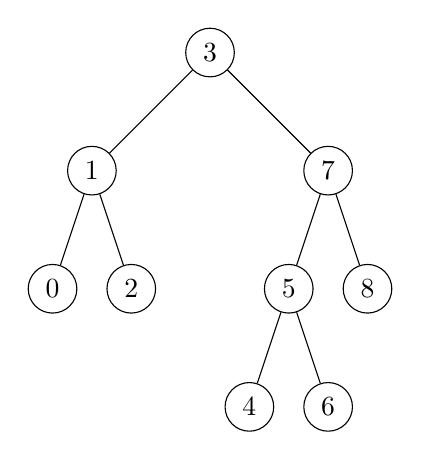
\begin{tikzpicture}
      [level 1/.style={sibling distance=30mm},
       level 2/.style={sibling distance=15mm},
       level 2/.style={sibling distance=10mm}]
      \tikzstyle{every node}=[circle,draw]
      \node{3}
      child{
        node{1}
        child{node{0}}
        child{node{2}}
      }
      child{
        node{7}
        child{
          node{5}
          child{node{4}}
          child{node{6}}
        }
        child{node{8}}
      };
    \end{tikzpicture} \hspace{4mm}
    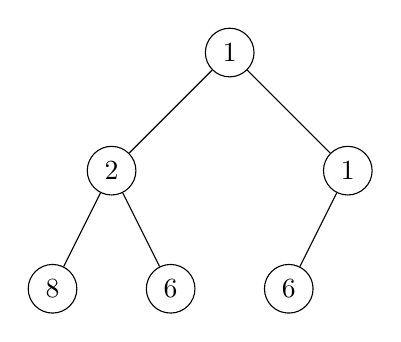
\begin{tikzpicture}
      [level 1/.style={sibling distance=30mm},
       level 2/.style={sibling distance=15mm}]
      \tikzstyle{every node}=[circle,draw]
      \node{1}
      child{
        node{2}
        child{node{8}}
        child{node{6}}
      }
      child{
        node{1}
        child{node{6}}
        child[missing]{node{k}}
      }
      ;
    \end{tikzpicture} \hspace{4mm}
    \begin{tikzpicture}[grow via three points={%
        one child at (0,-1.5) and two children at (0,-1.5) and (-1.5,-1.5)}]
      \tikzstyle{every node}=[circle,draw]
      \node at (0,0) {6}
      child{node{29}}
      child{
        node{14}
        child{
          node{38}
        }
      }
      child{
        node{8}
        child{node{17}}
        child{
          node{11}
          child{node{27}}
        }
      }
      ;
    \end{tikzpicture}
  \end{center}
  \caption{A binary search tree, a binary min-heap, and a binomial
    tree of rank $3$}
  \label{fig:trees}
\end{figure}

\begin{algorithm}[t]
  \begin{algorithmic}[1]  % comment [1] away to drop the line numbers
    \STATE \Function $f(n)$
    \IF[optional comment]{$n < 0$}
      \STATE $n \IsAssigned -2 \cdot n$ \COMMENT{optional comment}
    \ELSE[$n \geq 0$]
      \STATE $n \IsAssigned  3 \cdot n$
    \ENDIF
    \WHILE[optional comment]{$n > 0$}
      \STATE $n \IsAssigned n-1$
    \ENDWHILE
    \RETURN $n$
  \end{algorithmic}
  \caption{Silly algorithm}
  \label{algo:demo}
\end{algorithm}

% \vfill
% \noindent
% Feel free to report to the head teacher any other features that you
% would have liked to see discussed and exemplified in this template
% document.

\end{document}
